\documentclass[a4paper, oneside, nobib, notoc, justified]{tufte-book}

% Load packages
\usepackage{graphicx,xcolor}
\usepackage{tikz}
\pgfrealjobname{fig}
\usepackage{amsmath,amssymb}

% Colors
\definecolor{paired1}{HTML}{A6CEE3}

% Commands
\newcommand{\ft}[0]{\footnotesize}
\newcommand{\scs}[0]{\scriptsize}
\newcommand{\sm}[0]{\small}
\renewcommand{\vec}[1]{\ensuremath{\mathbf{#1}}}
\newcommand{\x}{\ensuremath{\vec{x}}}
\newcommand{\n}{\ensuremath{\vec{n}}}

\begin{document}
    \beginpgfgraphicnamed{fig2_01}
    \small
    \begin{tikzpicture}
        \draw (0,0) node [right] {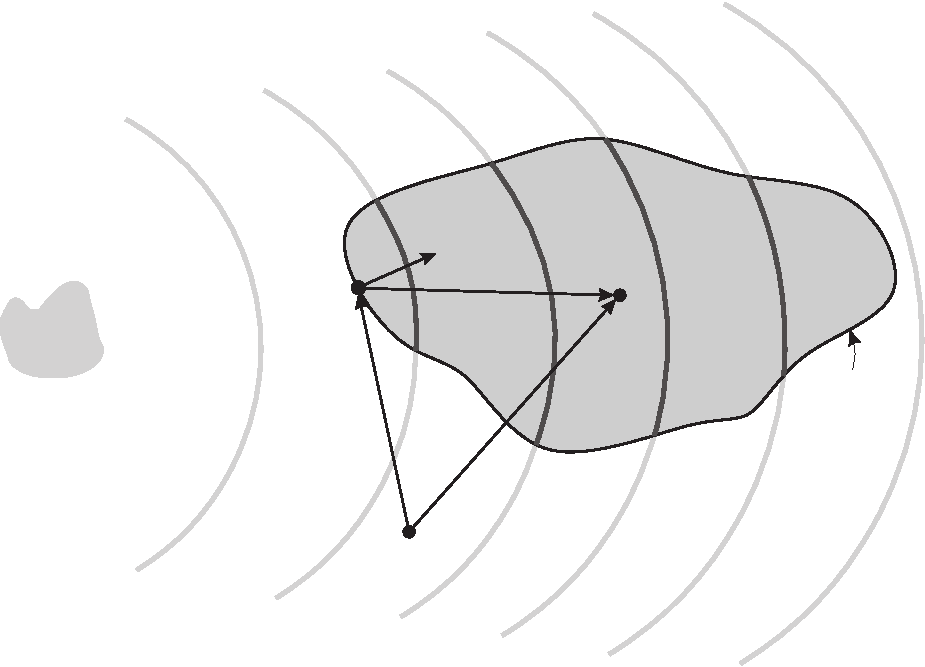
\includegraphics[scale=0.5]{src/kirchhoff_helmholtz_integral}};
        \draw (0.6,-0.6) node {virtual}; \draw (0.6,-0.9) node {source};
        \draw (6.9,-1.7) node {$S(\x,\omega)$}; \draw (2.84, 0.4) node {$\x_0$};
        \draw (3.9, 0.8) node {$\n$}; \draw (5.55, 0.35) node {$\x$};
        \draw (4.24, 0.0) node {$P(\x,\omega)$}; \draw (5.2, 0.9) node {$V$};
        \draw (7.3,-0.5) node {$\partial V$}; \draw (3.56,-1.9) node {$0$};
    \end{tikzpicture}
    \endpgfgraphicnamed
\end{document}
